\documentclass[a4paper]{article}
\usepackage[a4paper]{geometry}
\usepackage[utf8]{inputenc}
\usepackage{polski}
\usepackage[polish]{babel}
\usepackage[T1]{fontenc}
\usepackage{graphicx}
\usepackage{verbatim}
\usepackage{float}
\usepackage{minted}
\usepackage{microtype}
\usepackage{shortvrb}
\usepackage{amsmath}

\let\olditemize=\itemize \let\endolditemize=\enditemize \renewenvironment{itemize}{\olditemize \itemsep0em}{\endolditemize}

\title{TEMAT ĆWICZENIA: OpenGL – teksturowanie}
\author{Marcel Guzik}

\begin{document}
\section{Wprowadzenie}

Celem ćwiczenia jest pokazanie podstawowych technik teksturowania powierzchni
obiektów z wykorzystaniem mechanizmów biblioteki OpenGL z biblioteką GLUT. Na
przykładach zilustrowana będzie droga od przeczytania obrazu tekstury, do
nałożenia jaj fragmentów na poszczególne fragmenty modelu obiektu
trójwymiarowego.

\section{Teksturowanie powierzchni}

Teksturowanie polega na nanoszeniu na powierzchnie elementów modelu sceny
obrazów zadanych w postaci map bitowych. Obrazy te zwykle umieszczone są w
osobnych plikach. Ogólnie teksturowanie sprowadza się do trzech czynności. Po
pierwsze odczytania z pliku obrazu tekstury i umieszczeniu odpowiednich
danych w pamięci. Po drugie zdefiniowania tekstury, przez co należy rozumieć
określenie sposobu interpretacji odczytanych z pliku danych i wreszcie po
trzecie nałożenia tekstury na elementy modelu obiektu.

Proces nakładania dwuwymiarowej tekstury na trójwymiarowy obiekt nazywa się UV
mapping.

\begin{figure}[H]
    \centering
    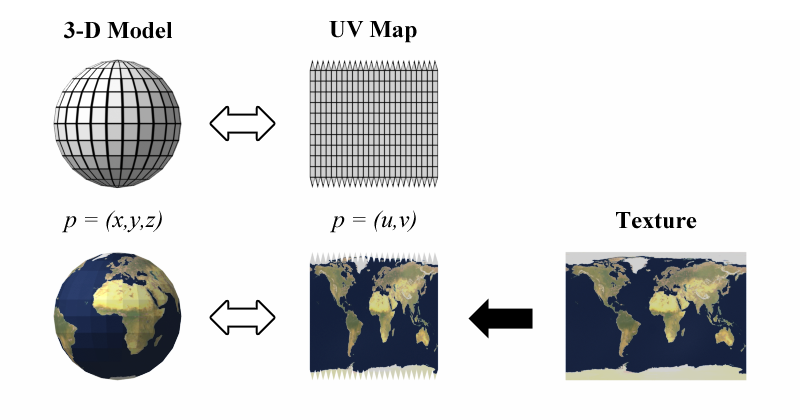
\includegraphics[width=0.5\textwidth]{uvmap}
    \caption{Nakładanie dwuwymiarowego obrazu na trójwymiarową sferę.}
\end{figure}

Program realizuje mapowanie kolorów obieku (diffuse mapping), metodę która (w
uproszczeniu) mapuje kolory z pliku graficznego bezpośrednio jako kolory
fragmentów rysowanych obiektów. Dostępne jest także m.in. mapowanie wypukłości,
mapowanie normalnych, mapowanie odbić zwierciadlanych, etc. Wszystkie te
techniki używają tekstur do określania poziomów tych parametrów niezależnie od
ilości i pozycji wierzchołków.

\begin{figure}[H]
    \centering
    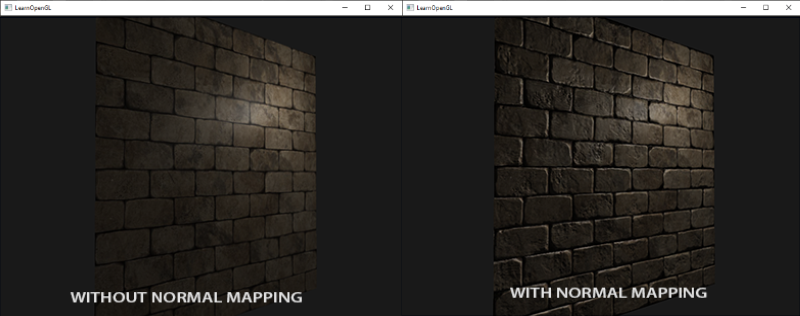
\includegraphics[width=\textwidth]{normalmapping}
    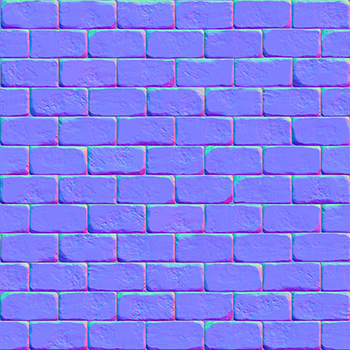
\includegraphics[width=0.3\textwidth]{normal_mapping_normal_map}

    \caption{Przykład zastosowania metody normal mapping. Powyżej przykład przed
        i po zaaplikowaniu tekstury. Poniżej zastosowana tekstura.}
\end{figure}


\section{Realizacja programu}

\subsection{Wczytywanie danych obrazu}

Aby wyświetlić teksturę na rysowanych obiektach, należy najpierw wczytać ją z
pliku. Posłuży do tego funkcja \mintinline{C}{LoadTGAImage()} wczytująca nasz
obraz w formacie TGA.

\subsection{Inicjalizacja}

W funkcji \mintinline{c}{init()} pojawił się następujący kod:

\begin{minted}{c}
    GLint ImWidth, ImHeight, ImComponents;
    GLenum ImFormat;
    GLbyte* texture = LoadTGAImage("tekstury/P4_t.tga", &ImWidth, &ImHeight,
        &ImComponents, &ImFormat);
    glTexImage2D(GL_TEXTURE_2D, 0, ImComponents, ImWidth, ImHeight,
        0, ImFormat, GL_UNSIGNED_BYTE, texture);
    glTexEnvi(GL_TEXTURE_ENV, GL_TEXTURE_ENV_MODE, GL_MODULATE);
    glTexParameteri(GL_TEXTURE_2D, GL_TEXTURE_MIN_FILTER, GL_LINEAR);
    glTexParameteri(GL_TEXTURE_2D, GL_TEXTURE_MAG_FILTER, GL_LINEAR);
    free(texture);
\end{minted}

Wartości kolorów pikseli obrazu są wczytywane przez funkcję
\mintinline{c}{LoadTGAImage()} i umieszczane w tablicy \verb|texture|.
Następnie funkcja \verb|glTexImage2D| tworzy teksturę z wczytanego obrazu.
Funkcja przyjmuje następujące argumenty:

\begin{itemize}
    \item \verb|GL_TEXTURE_2D|: \textbf{target} - Rodzaj definiowanej tekstury,
          zawsze powinno być \verb|GL_TEXTURE_2D|

    \item \verb|0|: \textbf{level} - Poziom szczegółowości. Jest ustawiany na 0
          gdy mipmapy nie są stosowane, gdy mipmapy są używane level jest liczbą
          określająca poziom redukcji obrazu tekstury.

    \item \verb|ImComponents|: \textbf{components} - Ilość używanych składowych
          koloru, liczba od 1 do 4.

    \item \verb|ImWidth|: \textbf{width} - Szerokosć obrazu tekstury, zawsze
          jest potegą liczby 2, może być powiększona o szerokość tak zwanej
          ramki tekstury

    \item \verb|ImHeight|: \textbf{height} - Wysokość obrazu tekstury, zawsze
          jest potęgą liczby 2, może być powiększona o szerokość ramki tekstury.

    \item \verb|0|: \textbf{border} - Szerokość ramki tekstury, może wynosić 0,
          1 lub 2

    \item \verb|ImFormat|: \textbf{format} - Format danych obrazu tekstury,
          określa co opisują dane, czy są indeksami kolorów czy ich składowymi
          (np. R, G, B) i w jakiej są podane kolejności.

    \item \verb|GL_UNSIGNED_BYTE|: \textbf{type} - Typ danych dla punktów obrazu
          tekstury, określa jak kodowane są dane, istnieje możliwość używania
          różnych formatów liczb, od 8 bitowych liczb stałoprzecinkowych, do 32
          bitowych liczb zmiennoprzecinkowych.

    \item \verb|texture|: \textbf{pixels} - Tablica o rozmiarze $width \times
              height \times components$, w ktorej znajdują się dane z obrazem
          tekstury.
\end{itemize}

Następnie kolejno:

\begin{enumerate}
    \item Za pomocą funkcji \verb|glTexEnvi()| ustawiamy funkcję teksturującą
          jako \verb|GL_MODULATE|. Funkcja teksturująca określa jak łączyć kolor
          obrazu tekstury z kolorem obrazu ekranu. \verb|GL_MODULATE| oznacza że
          kolor piksela ekranu jest mnożony przez kolor piksela tekstury,
          następuje w ten sposób mieszanie barw tekstury i tego co jest
          teksturowane.

    \item Za pomocą funkcji \verb|glTexParameteri()| określamy algortm dodawania
          nowych piksel w przypadku, gdy w obrazie tekstury jest za mało punktów
          aby wypełnić obraz teksturowanego elementu oraz usuwania pikseli, gdy
          w obrazie tekstury jest ich za dużo. W obu przypadkach stosujemy
          \verb|GL_LINEAR| co oznacza, że w przypadku potrzeby powiększenia lub
          pomniejszenia tekstury będziemy stosować interpolację liniową.
\end{enumerate}

\subsection{Definiowanie współrzędnych tekstury dla wierzchołków}

Do określania współrzędnych tekstury dla wierzchołków wykorzystano funkcję
\verb|glTexCoord2f|. Przyjmuje ona jako argumenty liczby zmiennoprzecinkowe
\verb|u| oraz \verb|v|, oznaczające odpowiednio pozycję wierzchołka na teksturze
wzdłuż osi x i y.

Przykładowo funkcja rysująca wierzchołki jaja wygląda w następujący sposób:

\begin{minted}{c}
void drawVertexTextured(int u, int v) {
    glNormal3fv(normals[u][v]);
    glTexCoord2f((float)v / (N-1), (float)u / (N-1));
    glVertex3fv(points[u][v]);
}
\end{minted}

\subsection{Back-face culling}

Aby nie teksturować niewidocznych dla obserwatora powierzchni wewnątrz obiektów,
stosuje się mechanizm back-face culling. Mechanizm ten określa czy powierzchnia
ustawiona jest do obserwatora przodem lub tyłem i teksturuje ją tylko jeśli jest
ustawiona przodem. Kierunek jest ustalany na podstawie kolejności rysowania
wierzchołków stanowiących tą powierzchnię, tzn. czy są rysowane zgodnie z
kierunkiem wskazówek zegara lub w kierunku przeciwnym. Domyślnie powierzchnie
rysowane w kierunku przeciwnym kierunkowi wskazówek zegara są określane jako
stojące przodem.

\begin{figure}[H]
    \centering
    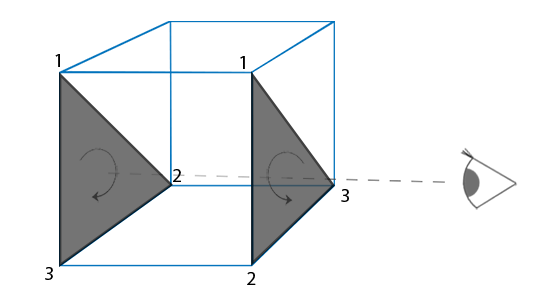
\includegraphics[width=0.6\textwidth]{draworder}
    \caption{Z punktu widzenia obserwatora wierzchołki stanowiące ściany po
        przeciwnych stronach sześcianu będą rysowane w odwrotnych kierunkach.}
\end{figure}

W programie proces uruchamiany jest przez funkcję \verb|glEnable(GL_CULL_FACE)|.

\begin{minted}{c}
void drawPyramid(float height) {
    glEnable(GL_CULL_FACE);
    glBegin(GL_QUADS);

    // ...

    glEnd();
    glDisable(GL_CULL_FACE);
}
\end{minted}

\begin{figure}[H]
    \centering
    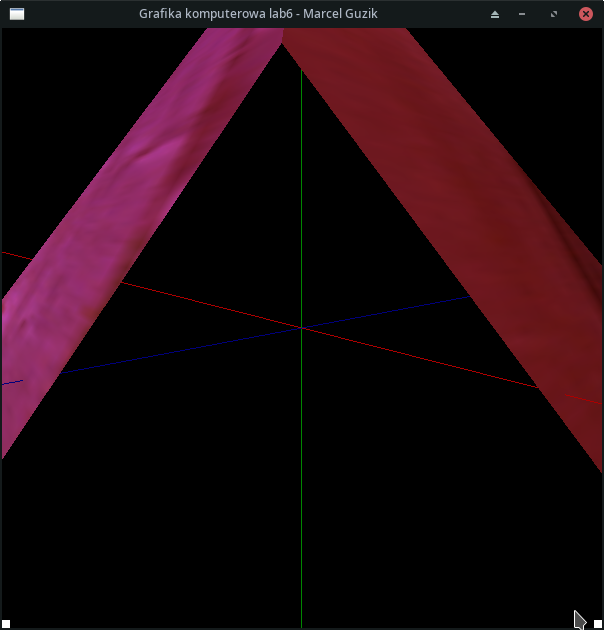
\includegraphics[width=0.5\textwidth]{backfaceculling}
    \caption{Mechanizm back-face culling pozwala na wyeliminowanie ścian
        wewnętrznych obiektów z procesu teksturowania i zaoszczędzenie mocy
        obliczeniowej.}
\end{figure}


\section{Podsumowanie}

\begin{figure}[H]
    \centering
    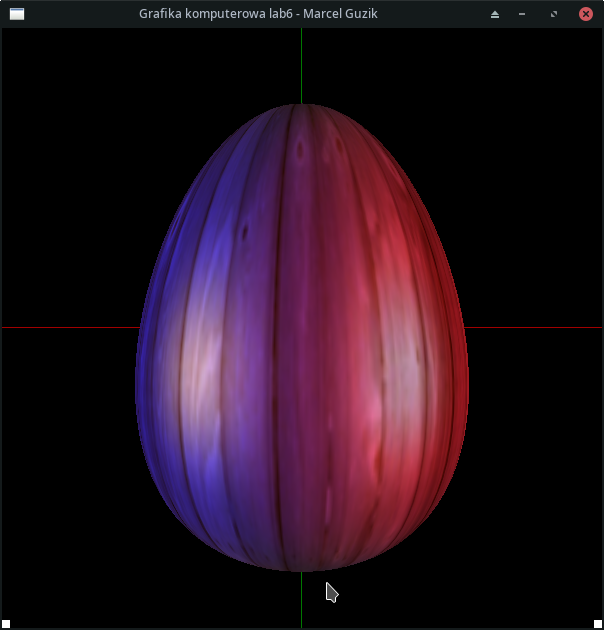
\includegraphics[width=0.3\textwidth]{egg}
    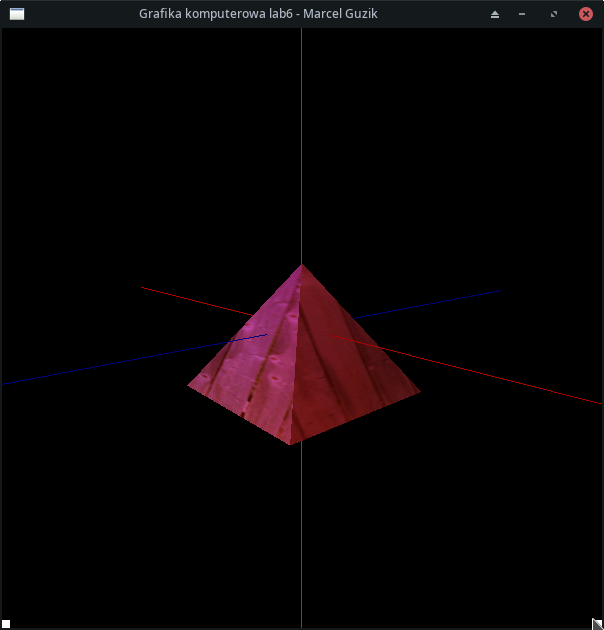
\includegraphics[width=0.3\textwidth]{pyramid}
    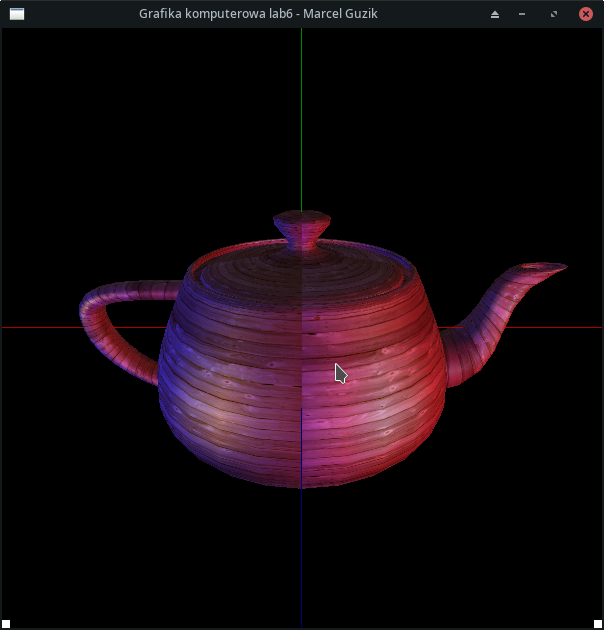
\includegraphics[width=0.3\textwidth]{teapot}

    \caption{Finalna wersja programu teksturująca obiekty.}
\end{figure}

Zadanie zaprezentowało możliwości teksturowania oraz mechanizmu back-face
culling w bibliotece OpenGL.

\end{document}